\documentclass{article}

\usepackage{amsmath,amssymb}
\usepackage{tikz}
\usepackage{xcolor}
\usepackage[left=2.1cm,right=3.1cm,bottom=3cm,footskip=0.75cm,headsep=0.5cm]{geometry}
\usepackage{enumerate}
\usepackage{enumitem}

\usepackage[utf8]{inputenc}

\renewcommand*{\arraystretch}{1.4}

\title{\textbf{Einführung in die Informatik, Übung 5}}
\author{\textsc{Henry Haustein}}
\date{}

\begin{document}
	\maketitle
	
	\section*{Aufgabe 5.1}
	
	\begin{enumerate}[label=(\alph*)]
		\item Gewichtsmatrix
		\begin{align}
		\begin{pmatrix}
		\infty & 60 & 20 & 10 & \infty & \infty \\
		\infty & \infty & 20 & \infty & 10 & \infty \\
		30 & \infty & \infty & \infty & \infty & 30 \\
		\infty & \infty & \infty & \infty & 70 & 50 \\
		\infty & \infty & \infty & 40 & \infty & 30 \\
		\infty & \infty & \infty & 20 & \infty & \infty \\
		\end{pmatrix}\notag
		\end{align}
		\item \textsc{Dijkstra}'s Algorithmus
		\begin{center}
			\begin{tabular}{c|ccccccc}
				\textbf{Iteration} & $S$ & $v_1$ & $D(b)$ & $D(c)$ & $D(d)$ & $D(e)$ & $D(f)$ \\
				\hline
				0 & $\{a\}$ & & 60 & 20 & \textcolor{red}{10} & $\infty$ & $\infty$ \\
				1 & $\{a,d\}$ & $d$ & 60 & \textcolor{red}{20} & 10 & 80 & 60 \\
				2 & $\{a,d,c\}$ & $c$ & 60 & 20 & 10 & 80 & \textcolor{red}{50} \\
				3 & $\{a,d,c,f\}$ & $f$ & \textcolor{red}{60} & 20 & 10 & 80 & 50 \\
				4 & $\{a,d,c,f,b\}$ & $b$ & 60 & 20 & 10 & \textcolor{red}{70} & 50 \\
				5 & $\{a,d,c,f,b,e\}$ & $e$ & 60 & 20 & 10 & 70 & 50 \\
			\end{tabular}
		\end{center}
	\end{enumerate}
	
	\section*{Aufgabe 5.2}
	
	Zahlen in den einzelnen Knoten sind die Knotengrade
	\begin{enumerate}[label=(\alph*)]
		\item ohne Waldschlösschenbrücke: alle Knotengrade sind gerade $\Rightarrow$ es gibt einen Eulerkreis $\Rightarrow$ Brückenproblem hat eine Lösung
		\begin{center}
			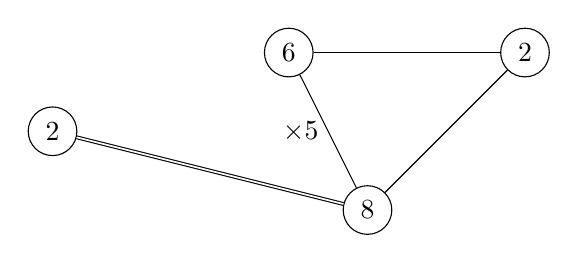
\begin{tikzpicture}
			\node[circle,draw=black, fill=white] (1) at (0,0) {2};
			\node[circle,draw=black, fill=white] (2) at (3,1) {6};
			\node[circle,draw=black, fill=white] (3) at (4,-1) {8};
			\node[circle,draw=black, fill=white] (4) at (6,1) {2};
			
			\draw[double] (1) -- (3);
			\draw (3) to node[midway,left] {$\times$5} (2);
			\draw (2) -- (4);
			\draw (3) -- (4);
			\end{tikzpicture}
		\end{center}
		\item mit Waldschlösschenbrücke: nicht alle Knotengrade sind gerade $\Rightarrow$ es gibt keinen Eulerkreis $\Rightarrow$ Brückenproblem hat keine Lösung
		\begin{center}
			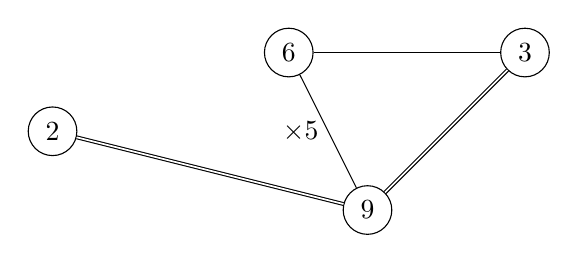
\begin{tikzpicture}
			\node[circle,draw=black, fill=white] (1) at (0,0) {2};
			\node[circle,draw=black, fill=white] (2) at (3,1) {6};
			\node[circle,draw=black, fill=white] (3) at (4,-1) {9};
			\node[circle,draw=black, fill=white] (4) at (6,1) {3};
			
			\draw[double] (1) -- (3);
			\draw (3) to node[midway,left] {$\times$5} (2);
			\draw (2) -- (4);
			\draw[double] (3) -- (4);
			\end{tikzpicture}
		\end{center}
	\end{enumerate}
	
	\section*{Aufgabe 5.3}
	
	\begin{enumerate}[label=(\alph*)]
		\item Kantenzahl: 17, Knotenzahl: 7 $\Rightarrow$ $17\not\le 3\cdot 7-6$ $\Rightarrow$ nicht planar
		\item nicht planar (zumindest vom Gefühl her)
	\end{enumerate}
	
	\section*{Aufgabe 5.4}
	\begin{center}
		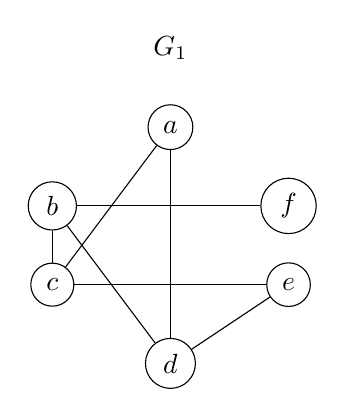
\begin{tikzpicture}
		\node[circle,draw=black, fill=white] (a) at (0,0) {$a$};
		\node[circle,draw=black, fill=white] (b) at (-1.5,-1) {$b$};
		\node[circle,draw=black, fill=white] (c) at (-1.5,-2) {$c$};
		\node[circle,draw=black, fill=white] (d) at (0,-3) {$d$};
		\node[circle,draw=black, fill=white] (e) at (1.5,-2) {$e$};
		\node[circle,draw=black, fill=white] (f) at (1.5,-1) {$f$};
		
		\draw (a) -- (c);
		\draw (a) -- (d);
		\draw (b) -- (c);
		\draw (b) -- (d);
		\draw (b) -- (f);
		\draw (c) -- (e);
		\draw (d) -- (e);
		
		\node at (0,1) {$G_1$};
		\end{tikzpicture}
		\hspace*{1cm}
		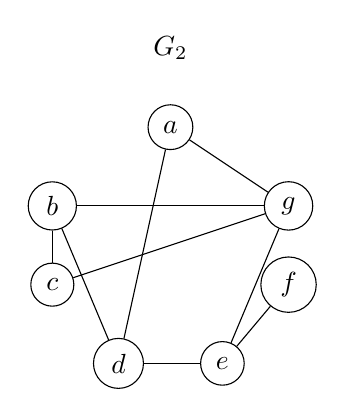
\begin{tikzpicture}
		\node[circle,draw=black, fill=white] (a) at (0,0) {$a$};
		\node[circle,draw=black, fill=white] (b) at (-1.5,-1) {$b$};
		\node[circle,draw=black, fill=white] (c) at (-1.5,-2) {$c$};
		\node[circle,draw=black, fill=white] (d) at (-0.66,-3) {$d$};
		\node[circle,draw=black, fill=white] (e) at (0.66,-3) {$e$};
		\node[circle,draw=black, fill=white] (f) at (1.5,-2) {$f$};
		\node[circle,draw=black, fill=white] (g) at (1.5,-1) {$g$};
		
		\draw (a) -- (d);
		\draw (a) -- (g);
		\draw (b) -- (c);
		\draw (b) -- (d);
		\draw (b) -- (g);
		\draw (c) -- (g);
		\draw (d) -- (e);
		\draw (e) -- (f);
		\draw (e) -- (g);
		
		\node at (0,1) {$G_2$};
		\end{tikzpicture}
		\hspace*{1cm}
		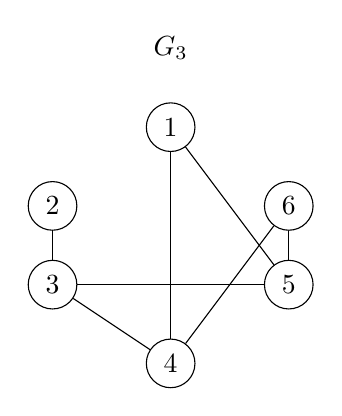
\begin{tikzpicture}
		\node[circle,draw=black, fill=white] (1) at (0,0) {1};
		\node[circle,draw=black, fill=white] (2) at (-1.5,-1) {2};
		\node[circle,draw=black, fill=white] (3) at (-1.5,-2) {3};
		\node[circle,draw=black, fill=white] (4) at (0,-3) {4};
		\node[circle,draw=black, fill=white] (5) at (1.5,-2) {5};
		\node[circle,draw=black, fill=white] (6) at (1.5,-1) {6};
		
		\draw (1) -- (5);
		\draw (1) -- (4);
		\draw (3) -- (5);
		\draw (3) -- (4);
		\draw (3) -- (2);
		\draw (5) -- (6);
		\draw (4) -- (6);
		
		\node at (0,1) {$G_3$};
		\end{tikzpicture}
	\end{center}
	\begin{enumerate}[label=(\alph*)]
		\item $G_1$ ist isomorph zu $G_3$ ($G_1\overset{\sim}{=}G_3$) mit folgender Bijektion
		\begin{center}
			\begin{tabular}{c|cccccc}
				$x$ & $a$ & $b$ & $c$ & $d$ & $e$ & $f$ \\
				\hline
				$f(x)$ & 1 & 3 & 5 & 4 & 6 & 2
			\end{tabular}
		\end{center}
		\item $G_1$ und damit auch $G_3$ sind 2-färbbar, $G_2$ ist es nicht, da es einen Kreis ungerader Länge enthält: $b\to g\to c\to b$
		\begin{center}
			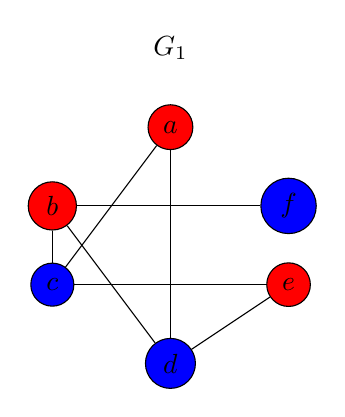
\begin{tikzpicture}
			\node[circle,draw=black, fill=red] (a) at (0,0) {$a$};
			\node[circle,draw=black, fill=red] (b) at (-1.5,-1) {$b$};
			\node[circle,draw=black, fill=blue] (c) at (-1.5,-2) {$c$};
			\node[circle,draw=black, fill=blue] (d) at (0,-3) {$d$};
			\node[circle,draw=black, fill=red] (e) at (1.5,-2) {$e$};
			\node[circle,draw=black, fill=blue] (f) at (1.5,-1) {$f$};
			
			\draw (a) -- (c);
			\draw (a) -- (d);
			\draw (b) -- (c);
			\draw (b) -- (d);
			\draw (b) -- (f);
			\draw (c) -- (e);
			\draw (d) -- (e);
			
			\node at (0,1) {$G_1$};
			\end{tikzpicture}
			\hspace*{1cm}
			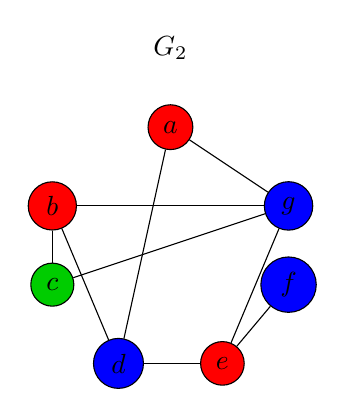
\begin{tikzpicture}
			\node[circle,draw=black, fill=red] (a) at (0,0) {$a$};
			\node[circle,draw=black, fill=red] (b) at (-1.5,-1) {$b$};
			\node[circle,draw=black, fill=green!80!black] (c) at (-1.5,-2) {$c$};
			\node[circle,draw=black, fill=blue] (d) at (-0.66,-3) {$d$};
			\node[circle,draw=black, fill=red] (e) at (0.66,-3) {$e$};
			\node[circle,draw=black, fill=blue] (f) at (1.5,-2) {$f$};
			\node[circle,draw=black, fill=blue] (g) at (1.5,-1) {$g$};
			
			\draw (a) -- (d);
			\draw (a) -- (g);
			\draw (b) -- (c);
			\draw (b) -- (d);
			\draw (b) -- (g);
			\draw (c) -- (g);
			\draw (d) -- (e);
			\draw (e) -- (f);
			\draw (e) -- (g);
			
			\node at (0,1) {$G_2$};
			\end{tikzpicture}
			\hspace*{1cm}
			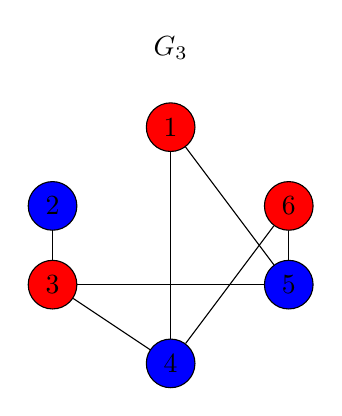
\begin{tikzpicture}
			\node[circle,draw=black, fill=red] (1) at (0,0) {1};
			\node[circle,draw=black, fill=blue] (2) at (-1.5,-1) {2};
			\node[circle,draw=black, fill=red] (3) at (-1.5,-2) {3};
			\node[circle,draw=black, fill=blue] (4) at (0,-3) {4};
			\node[circle,draw=black, fill=blue] (5) at (1.5,-2) {5};
			\node[circle,draw=black, fill=red] (6) at (1.5,-1) {6};
			
			\draw (1) -- (5);
			\draw (1) -- (4);
			\draw (3) -- (5);
			\draw (3) -- (4);
			\draw (3) -- (2);
			\draw (5) -- (6);
			\draw (4) -- (6);
			
			\node at (0,1) {$G_3$};
			\end{tikzpicture}
		\end{center}
		\item Bipartit und 2-färbbar sind das gleiche $\Rightarrow$ selbe Antwort wie bei (b)
	\end{enumerate}
\end{document}